\documentclass[11pt]{article}

\usepackage{graphicx}			% Use this package to include images
\usepackage{amsmath}			% A library of many standard math expressions
\usepackage{amsfonts}
\usepackage[margin=1in]{geometry}% Sets 1in margins.
\usepackage{fancyhdr}			% Creates headers and footers
\usepackage{enumerate}          %These two package give custom labels to a list
\usepackage[shortlabels]{enumitem}
\usepackage{braket}
\usepackage{physics}
\usepackage{pgfplots}
\usepackage{tikz}
\usepackage{xcolor}
\usepackage{mathtools}
\usepackage{url}
\usepackage{listings}
\usepackage{geometry}

%% LISTINGS CONFIG %%

\definecolor{purple2}{RGB}{153,0,153} % there's actually no standard purple
\definecolor{green2}{RGB}{0,153,0} % a darker green

\renewcommand{\lstlistingname}{Code}

% Define MATLAB style
\lstset{
    language=Matlab,
    basicstyle=\ttfamily\small, % Font size and typewriter style
    keywordstyle=\color{blue}\bfseries, % Keywords in bold blue
    commentstyle=\color{green!60!black}\itshape, % Comments in italic green
    stringstyle=\color{red}, % Strings in red
    numbers=left, % Line numbers on the left
    numberstyle=\tiny\color{gray}, % Line number style
    stepnumber=1, % Line number increment
    numbersep=5pt, % Distance of line numbers from code
    backgroundcolor=\color{gray!10}, % Light gray background
    frame=single, % Box around the code
    rulecolor=\color{black}, % Frame color
    tabsize=4, % Tab size
    showspaces=false, % Do not show spaces as visible characters
    showstringspaces=false, % Do not show spaces in strings
    breaklines=true, % Automatic line breaking
    captionpos=b, % Caption at the bottom
}

\title{\textbf{ECE469 Homework 3}}
\author{Chase A. Lotito}
\date{\today}

\begin{document} %The writing for your homework should all come after this.

\maketitle

% QUESTION 1
\section*{Question 1}

Train SVM classifiers using a Gaussian Kernel based on MATLAB.

\smallskip
\textbf{Solution.}

% code from q1.m
\lstinputlisting[caption={q1.m}, label={code:q1}]{../q1/q1.m}

Code \ref{code:q1} utilizes a user-defined function to implement the Gaussian Kernel which can be referenced in Code \ref{code:mysigmoid}.


\begin{figure}[!h]
  \centering
  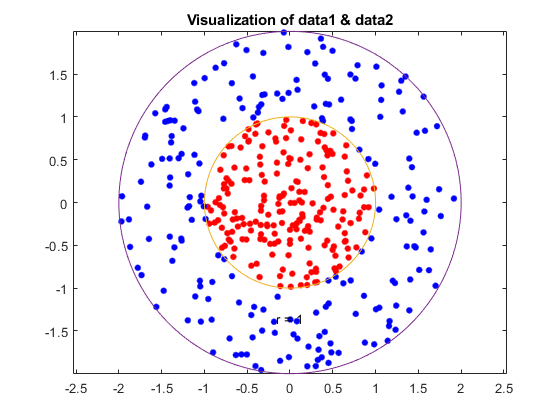
\includegraphics[width=0.75\textwidth]{../q1/data1_data2_visualization.png}
  \label{fig:q1_data_visual}
\end{figure}

\begin{figure}[!h]
  \centering
  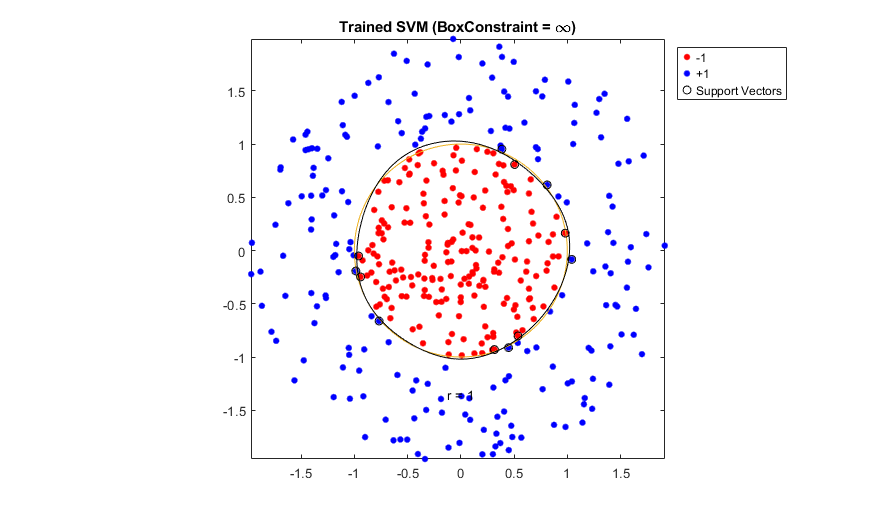
\includegraphics[width=1.0\textwidth]{../q1/trained_svm_inf.png}
  \label{fig:trained_svm_inf}
\end{figure}

\begin{figure}[!h]
  \centering
  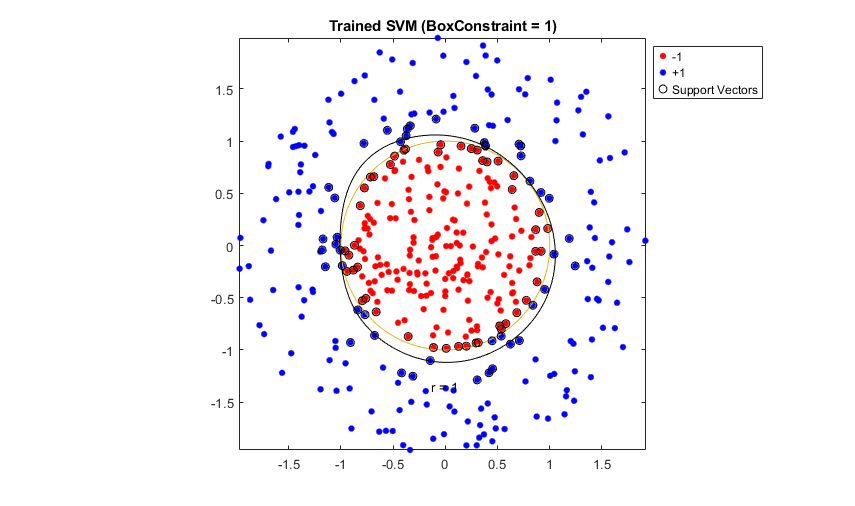
\includegraphics[width=1.0\textwidth]{../q1/trained_svm_1.png}
  \label{fig:trained_svm_1}
\end{figure}


For \(\texttt{BoxConstraint}=1\) the decision boundary is warped and we have more misclassifications. For \(\texttt{BoxConstraint}=\infty\), the decision boundary is nearly the unit circle, and there are barely any misclassifications.














\clearpage
% QUESTION 2
\section*{Question 2}

\textbf{Solution.}

% code from q2.m
\lstinputlisting[caption={q2.m}, label={code:q2}]{../q2/q2.m}


\begin{figure}[!h]
  \centering
  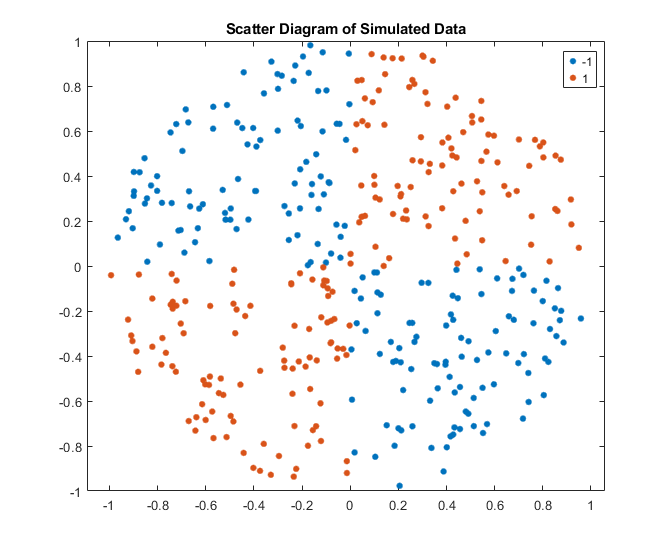
\includegraphics[width=1.0\textwidth]{../q2/scatter.png}
  \label{fig:scatter}
\end{figure}

\begin{figure}[!h]
  \centering
  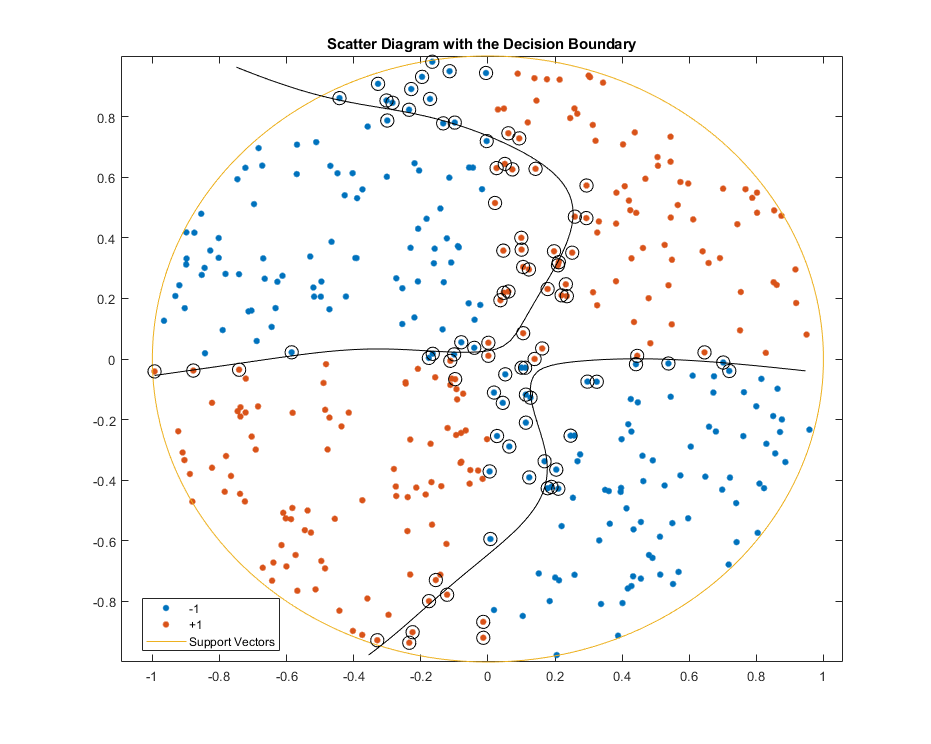
\includegraphics[width=1.0\textwidth]{../q2/scatter_dbound.png}
  \label{fig:scatter_gamma1}
\end{figure}


\begin{figure}[!h]
  \centering
  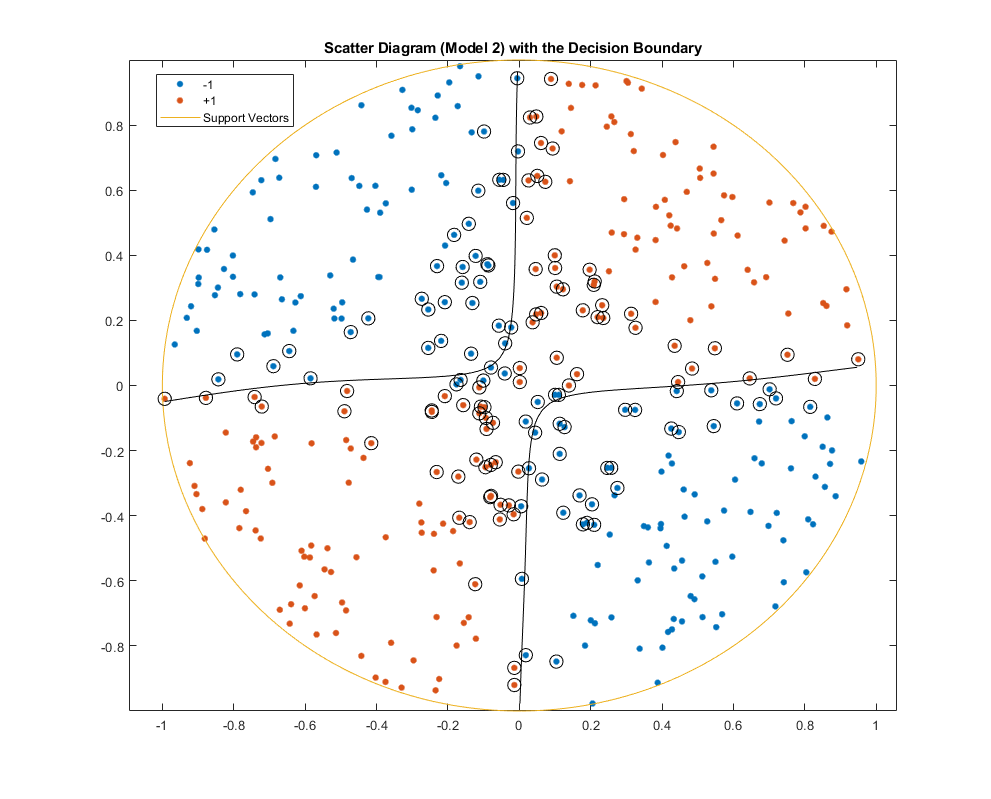
\includegraphics[width=1.0\textwidth]{../q2/scatter_dbound_model2.png}
  \label{fig:scatter_gamma05}
\end{figure}


\begin{figure}[!h]
  \centering
  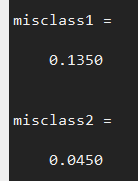
\includegraphics[width=0.25\textwidth]{../q2/misclass_rates.png}
  \label{fig:misclassrates}
\end{figure}

For Gaussian Kernel, \(\texttt{gamma}=1\) (Model 1) misclassification rate is 13.5\%, \(\texttt{gamma}=0.5\) (Model 2) misclassification rate is 4.5\%.












\clearpage
% QUESTION 3
\section*{Question 3}

\textbf{Solution.}

% code from q3.m
\lstinputlisting[caption={q3.m}, label={code:q3}]{../q3/q3.m}



\clearpage
% QUESTION 4
\section*{Question 4}

\textbf{Solution.}

% code from q4.m
\lstinputlisting[caption={q4.m}, label={code:q4}]{../q4/q4.m}



\begin{figure}[!h]
  \centering
  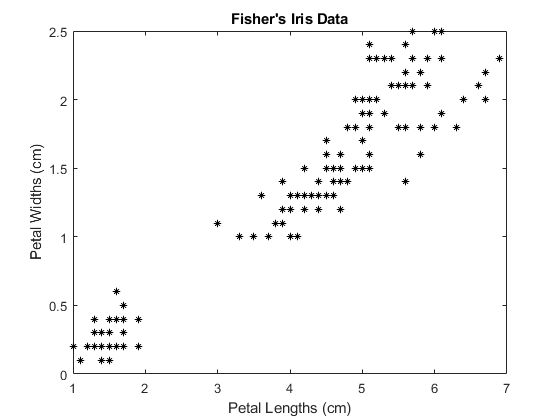
\includegraphics[width=0.75\textwidth]{../q4/fisheriris_unclustered.png}
  \label{fig:fishunclust}
\end{figure}


\begin{figure}[!h]
  \centering
  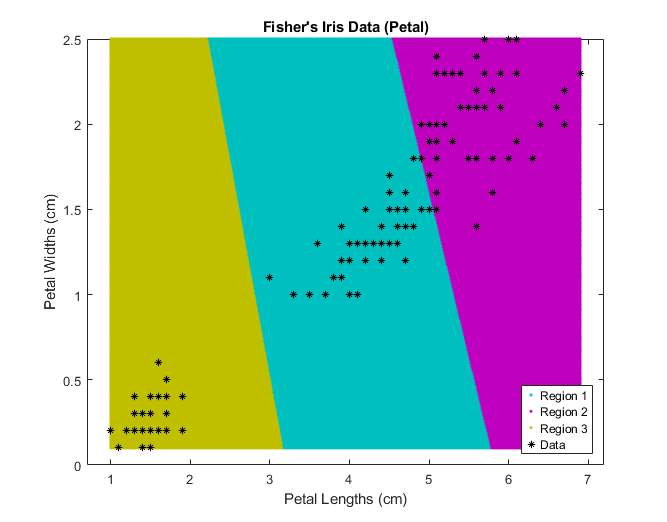
\includegraphics[width=0.75\textwidth]{../q4/fisheriris_clustered.png}
  \label{fig:fishclust}
\end{figure}


\begin{figure}[!h]
  \centering
  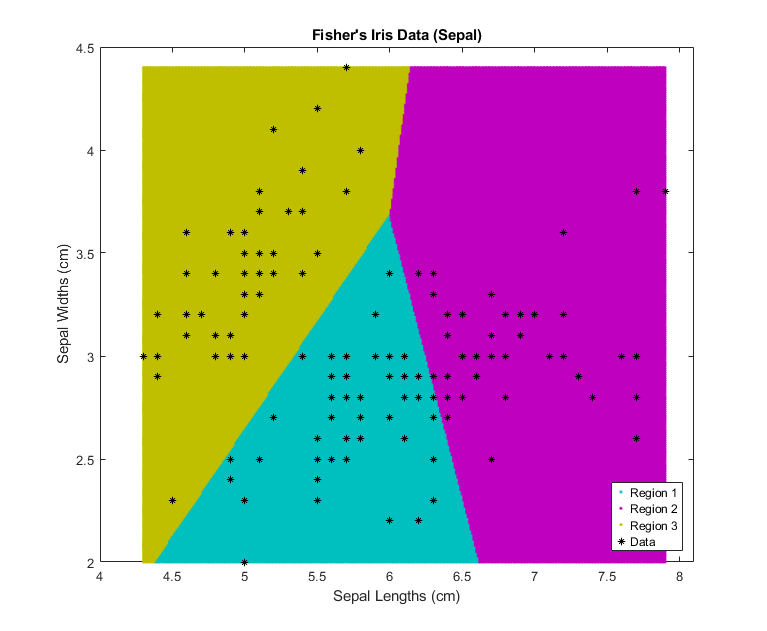
\includegraphics[width=0.75\textwidth]{../q4/sepal_fisheriris_clustered.png}
  \label{fig:sepalclust}
\end{figure}





\clearpage
% QUESTION 5
\section*{Question 5}

\textbf{Solution.}

% code from q5.m
\lstinputlisting[caption={q5.m}, label={code:q5}]{../q5/q5.m}


\begin{figure}[!h]
  \centering
  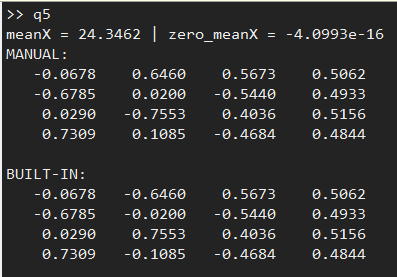
\includegraphics[width=0.75\textwidth]{../q5/q5_log.png}
  \label{fig:q5log}
\end{figure}

\clearpage
(ii)
\begin{figure}[!h]
  \centering
  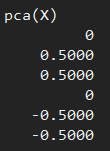
\includegraphics[width=0.35\textwidth]{../q5/pcaX.png}
  \label{fig:pcaX}
\end{figure}



\clearpage
% QUESTION 6
\section*{Question 6}

\textbf{Solution.}

% code from q6.m
\lstinputlisting[caption={q6.m}, label={code:q6}]{../q6/q6.m}

\begin{figure}[!h]
  \centering
  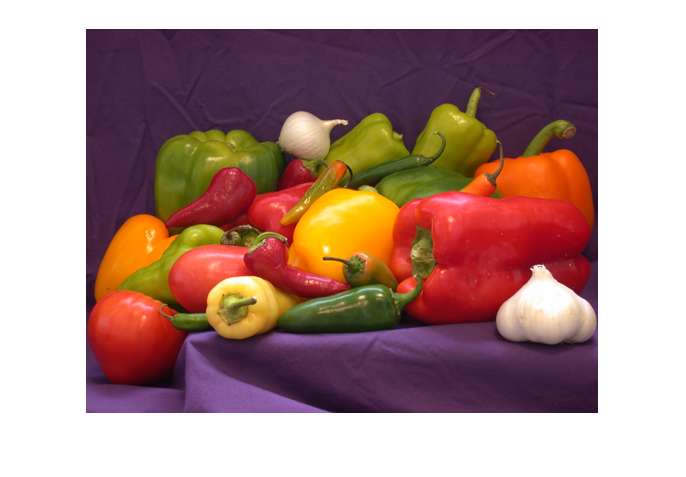
\includegraphics[width=0.75\textwidth]{../q6/peppers.png}
  \label{fig:pep}
\end{figure}


\begin{figure}[!h]
  \centering
  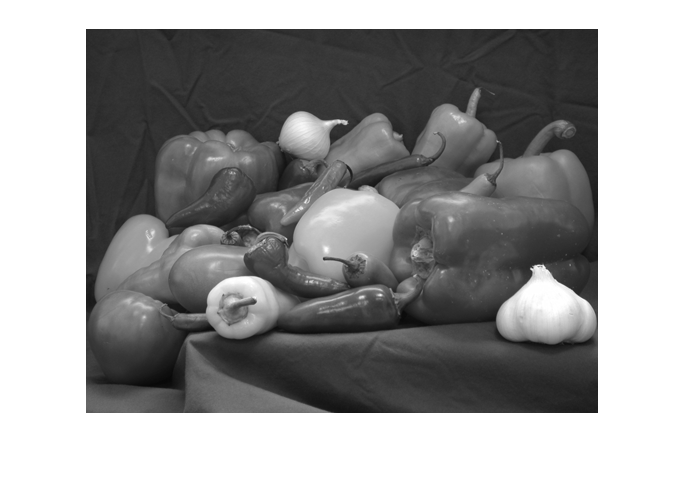
\includegraphics[width=0.75\textwidth]{../q6/peppers_gray.png}
  \label{fig:pepgray}
\end{figure}

\begin{figure}[!h]
  \centering
  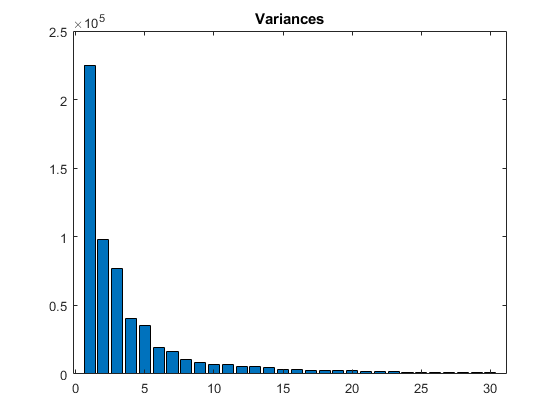
\includegraphics[width=0.75\textwidth]{../q6/variances.png}
  \label{fig:var}
\end{figure}


\begin{figure}[!h]
  \centering
  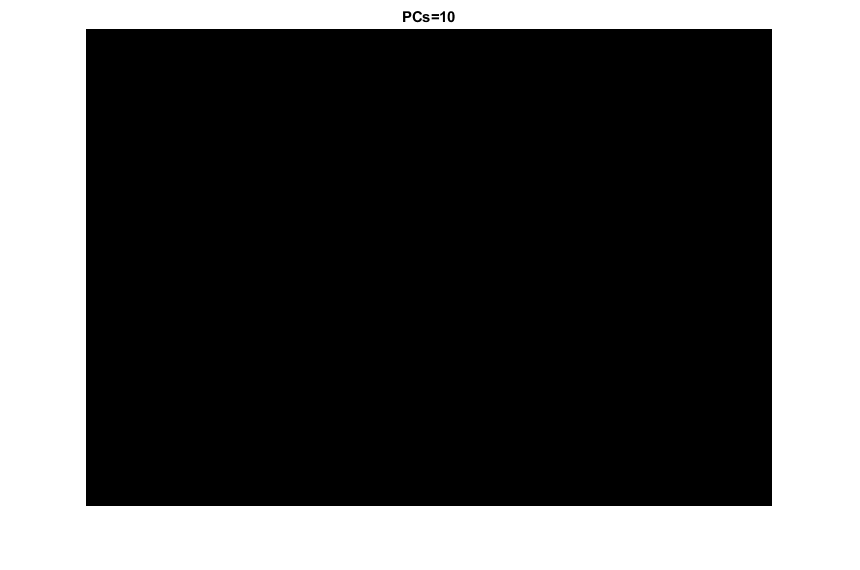
\includegraphics[width=0.75\textwidth]{../q6/compressed_10.png}
  \label{fig:comp10}
\end{figure}

\begin{figure}[!h]
  \centering
  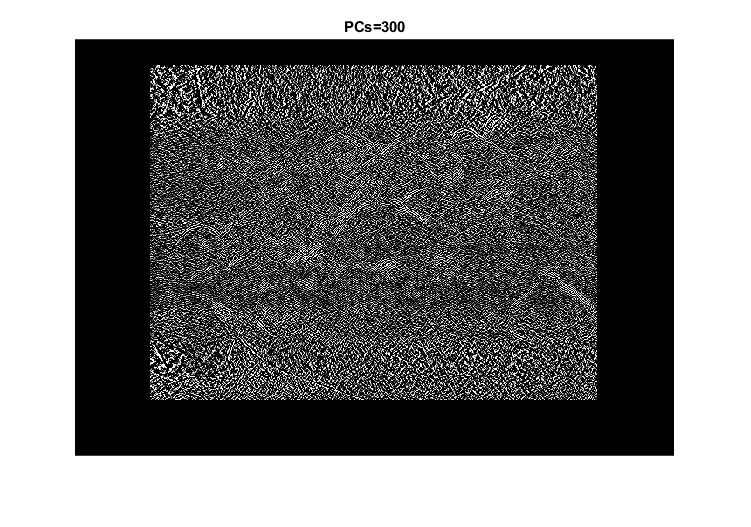
\includegraphics[width=0.75\textwidth]{../q6/compressed_300.png}
  \label{fig:comp300}
\end{figure}

\begin{figure}[!h]
  \centering
  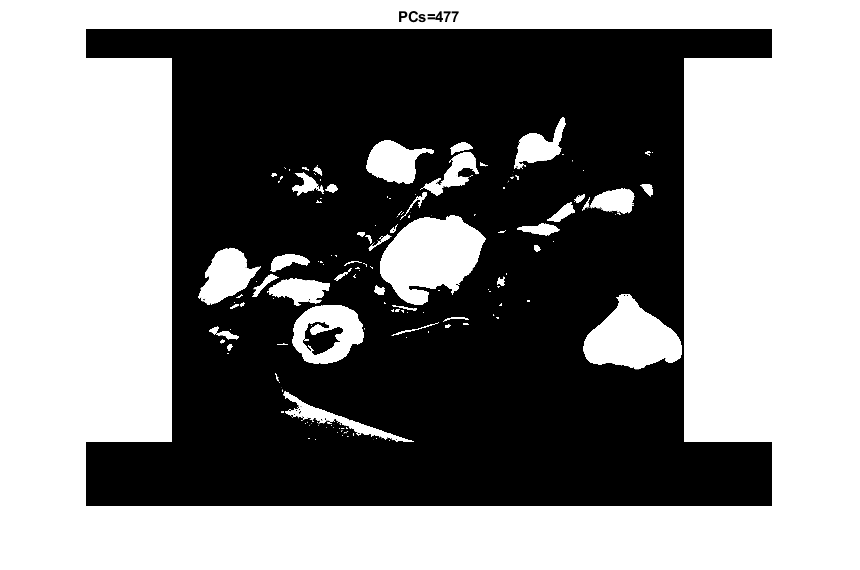
\includegraphics[width=0.75\textwidth]{../q6/compressed_477.png}
  \label{fig:comp477}
\end{figure}

The image quality for the compressed PCA images is very low, but for \(\texttt{PCs=477}\) you can see strong outlines of the peppers.


\clearpage
% QUESTION 7
\section*{Question 7}

\textbf{Solution.}

% code from q7.py
\lstinputlisting[caption={q7.py}, label={code:q7}]{../q7/q7.py}


% APPENDIX
\clearpage
\section*{APPENDIX A: Auxillary Code}

The following codes was used to implement the Gaussian Kernel for Support Vector Machines (SVM).

\lstinputlisting[caption={mysigmoid.m}, label={code:mysigmoid}]{../q2/mysigmoid.m}


\lstinputlisting[caption={mysigmoid\_2.m}, label={code:mysigmoid2}]{../q2/mysigmoid_2.m}

\end{document}